\documentclass[conference,compsoc]{IEEEtran}
\usepackage{cite}
\usepackage{listings}
\usepackage{blindtext}
\usepackage{enumitem}
% for coding highlight
\usepackage{graphicx}
\usepackage[colorlinks=true,urlcolor=blue]{hyperref}
\usepackage{amsmath, amsthm, amssymb}
\usepackage{subfloat}
\usepackage{ulem}
\usepackage{indentfirst}
\usepackage{booktabs}
\usepackage{wrapfig,lipsum,booktabs}
\usepackage{array}
\usepackage{blindtext}
\usepackage{algorithm}  
\usepackage{algorithmicx}  
\usepackage{algpseudocode} 
\begin{document}
\title{
	CS140 Report: \\Dynamic Graph Connectivity in Polylogarithmic Worst Case Time
}


% author names and affiliations
% use a multiple column layout for up to three different
% affiliations
\author{
	\IEEEauthorblockN{He Wang, Zhiqiang Xie, Youmi Ma, Jianxiong Cai, Yuyang Rong}
	\IEEEauthorblockA{
		School of Information Science and Technology \\
		ShanghaiTech University \\
	}
}

\maketitle


\begin{abstract}
The dynamic graph connectivity problem is as follows: given a graph on a fixed nodes, there are three operations: insert, delete, query. The data structure of this paper can solve this problem in polylogarithmic worst case time per operation. And during the past 30 years, all the data structures for solving this problem have $\Theta(n)$ worst case time per operation. 
\\
In this paper, it presents a solution with $O(log^4n)$ per insertion, $O(log^5n)$ per deletion, $O(log\ n/log\ log n)$ per query. And it introduces a one-side error, which means when the answer to a query is "yes", it is totally correct, but when the answer to query is "no", it has a high probability to be the right answer. The data structure bases on the idea of cutset and does some improvements to find the replacement edge in the cutset. 
\end{abstract}
\section{Introduction}
This paper focuses on the dynamic connectivity problem. Given a graph $G=(V,E)$, where $V$ is a fixed set of n nodes, and there are three main operations as the following form:\\

$\centerdot$ Delete(e): Delete edge e from E.\\

$\centerdot$ Insert(e): Insert edge e into E.\\

$\centerdot$ Query(a,b): check if there is a path from a to b.\\


The goal of this paper is to minimize the cost of  the above operations. 

In the words of Patrascu and Thorup, it is "perhaps the most fundamental challenge in dynamic graph algorithms today".  Therefore, there are some previous works on it. In the past 30 years, some researchers did the improvements. In 1985, Frederickson introduced that a data structure which decomposes the spanning forest into a hierarchical structure of subtrees and as a result, this problem could be solved at worst cast time of $O(\sqrt m)$ 
In the 1995, Henzinger and King gave the first polylogarithmic amortized expected update time $O(log^3 n)$ and in the 2000, Thorup gave a randomized data structure with the $O(log\ n(log \ log n)^3)$ amortized update time. However, all these algorithms have the worst cast time $\tilde{O} (n)$.
It is worth to mention that this paper is the first solution who meets the lower bound of the dynamic connectivity problem And that is the reason why it wins the best paper award of SODA 2013.
\\
\\
$The$ $idea$: 
It is relatively easy to deal with edge insertion, but it is more difficult to find a replacement edge when a tree edge is deleted, separating the origin tree into two subtrees. And this paper noticed that each replacement edge has exactly one endpoint in a subtree; all other edges have 0 or 2. And there are two ways to implement it. One is to add the name of each edges to the values stored at both its endpoints and do the operation XOR of the values of each nodes in a tree. The other is that for each edge, assign one endpoint -1 or 1 randomly and the other endpoint to the remaining value, and then sum all points to approximate the size of the cut. Even though the data structure seems simple, it is a challenge to preserves sufficient independence of randomness over a number of updates.
\\
\\
$Main$ $results$


$\centerdot$  insertion: worst case $O(log^4n)$\\

$\centerdot$  deletion: worst case $O(log^5n)$\\

$\centerdot$  insertion: worst case $O(log\ n/log\ log n)$\\

Though, it introduces the False Negative error which means if the answer to a query is "yes", it is totally correct, but when the answer to query is "no", it is correct with probability 1-1/$n^c$ for c any constant.
\\

We will explain more related works in Section 2 and 3. In Section 2, we introduce the Boruvka tree and in Section 3, we give the basic introduction to ET-tree. In Section 4, we explain the data structure of this paper and show how to find a replacement edge in cut set and prove its correctness. In the Section 5, we explain the reason why it can be used to this algorithm. In the Section 6 and 7, we explain how the algorithms works and why it is correct and efficient. The applications and discussion follow in Section 8 and 9.

\section{Borůvka's algorithm}
\subsection{Original Algorithm}
Originally, Borůvka's algorithm is an algorithm for finding a minimum spanning forest in the given graph. The principle is that the algorithm keep connecting components with the cheapest edge between them (the edge with minimum wight).
\par
To be specific, the algorithm first initialize n components which only contain a single node, whose cheapest edge value W is set to inf. (n is the number of vertex in the graph). Then for each edge which containing different components, if the weight of the edge is smaller than either of the cheapest edge value W, it is added to the tree and those two components is connected with each other in the next iteration. 
The Pseudo code is shown following.

\subsection{Pseudo code}
For each connected component in the forest, it stores a value representing the cheapest edge weight in the component (W).
\begin{algorithm}[H]
\caption{Borůvka's algorith}
\begin{algorithmic}[1]
\State initial forest F to be one-vertex tree.
\While {F is not the maximum connected tree}:
	\For{ each edge uv (containing node u and v)}:
		\If {u, v belongs to different components}:
			\If {weight(uv) less than u.W }:
				\State set weight(uv) as the u.W
			\EndIf
			\If {weight(uv) less than v.W }:
				\State set weight(uv) as the v.W
			\EndIf
		\EndIf
	\EndFor
	\For {each updated edge uv} 
		\State connect u and v
		\State set its cheapest value to min(u.W,v.W)
	\EndFor
\EndWhile
\end{algorithmic}
\end{algorithm}
\subsection{Algorithm used in this work}
	In this paper, instead of using the cheapest edge each time, it randomly choose an edge to connect different components. The reason is that it does not need a minimum spanning forest, instead, it only need to obtain a forest with maximum-connectivity.

\section{ET-tree}
Euler tour representation technique  \cite{715896} is a milestone for a bunch of problems who can be interpreted in dynamic forests. It introduces a powerful way to dynamically link and cut tree data structure efficiently in constant number of operations. However, it's not flexible enough to handle different kind of queries.

Further, a more compact and general data structure Euler tour tree \cite{Henzinger:1995:RDG:225058.225269} (ET-tree) is proposed, which suggests to represent a given tree by keeping its Euler tour in a balanced binary search tree, keyed by the index in the tour. Differ to the oridinary Euler tour representation, it's more similar to an earlier idea called link-cut tree\cite{Sleator:1985:SBS:3828.3835} who guarantees operating in $O(\log n)$ time either. While link-cut trees are good for maintaining aggregates on paths of a tree (making it a good choice data structure in network flow algorithm), ET-trees are batter at keeping aggregate information on subtrees.
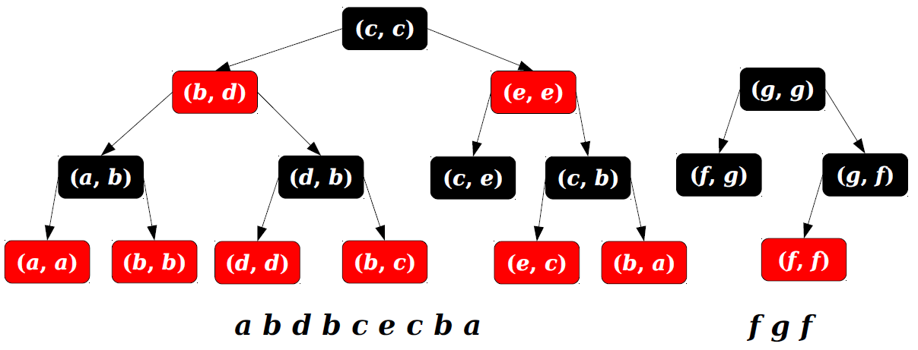
\includegraphics[height=3.2cm]{Pic/ET-tree.png}
\textbf{Properties:}
If each node in the graph has a value stored in $c$ words of length $O(\log n)$ ($c\leq \log n$ which can be treated as always holding) then: 
(1) a tree edge can be deleted or inserted in $O(c \log n)$ time;
(2) the sum of the values stored in the nodes of a given tree can be returned in $O(c)$ time; 
(3) a value at a node can be updated in $O(c \log n)$ time per word; 
(4) given a node $v$, the name of the tree $T(v)$ containing $v$ can be returned in $O(\log n)$ time. 
(5)The name of the tree can be obtained more quickly if one keeps an ET-tree of degree $\log n$ solely for this purpose. That is, it can be obtained in $O(\log n/ \log \log n)$ if one is willing to spend $O(\log^2 n)$ time doing an insertion or deletion of a tree edge.

In this paper, they presents the data structure with the help of ET-trees: store the selected trees in ET-tree, this Monte Carlo randomized algorithm roughly introduce a novel idea who operates in polylogarithmic worst case time to meet the bottom neck brought by ET-tree.

\section{Data Structure}
One of the major difficulties researchers often encounter with is the maintenance of a maximal spanning tree(or, maximal spanning forest, if the graph is not connected). Problems arise when we can $delete\{x,y\}$ operation to remove one edge $\{x,y\}$ which is a component of the MST or MSF, causing it relatively difficult to find a replacement edge. The novel idea and data structure from this paper coupe with this problem in a quite smart way, although introduced a low-probability false-negative error. The data structure, which from our point of view is one of the highlights of this paper, is called \textbf{Cutset}. \\
Here we refer to cutset as \textbf{edge} cutset. An edge cutset $S$ of graph $G=(V,E)$ contains a couple of edges $e=\{x,y\}$, where $x \in V_1,V_1 \subset V $ and $y \in V \backslash V_1$. A removal of any edge inside the cutset $S$ would disconnect the graph. \\
Authors of this paper defined the $cutset$ $problem$: Consider a forest $F$ of disjoint trees, not necessarily maximal, in graph $G$, where $G$ and $F$ are both dynamic. The goal is to maintain, for each non-maximal tree $T\in F$, an edge in the cutset of $(T,V\backslash T)$. Since every tree $T\in F$ itself is connected, every time we check for the $Query(a,b)$ problem('Is there a path between node $a$ and $b$?'), we only need to find a cut edge of $(T(a),T(b))$; Meanwhile, for the cutset problem, we are going to maintain a cutset of $(T,V\backslash T)$ for every $T \in F$, thus if we can solve the connectivity problem above if we can solve the cutset problem.\\
Generally speaking, cutset data structure deals with the following operations:\\\\
$Insert\{x,y\}$: Insert edge $\{x,y\}$ into graph $G$.\\
$Make \{x,y\}$ $a$ $tree$ $edge$: Join $T(x)$ and $T(y)$ together, by using the edge $\{x,y\}$.\\
$Delete\{x,y\}$: Delete edge $\{x,y\}$ from the graph $G$. If the edge is in $F$, remove it from $F$.\\
$Search(T)$: Return an edge in the cutset $(T,V\backslash T)$, if any.
\subsection{Construction of a cutset data structure}
For simplicity, we introduce first a cutset data structure where each cutset contains exactly one edge, since the construction of more complex cases are based on this trivial one. To construct such a data structure, there are mainly four steps.
\subsubsection*{Step 1} Encode each node $x \in V$ in binary, as shown in  Figure~\ref{fig:1}. Note these binary representations as $x_b$ where $b$ stands for binary, for each node.
\begin{figure}[h]
	\centering
	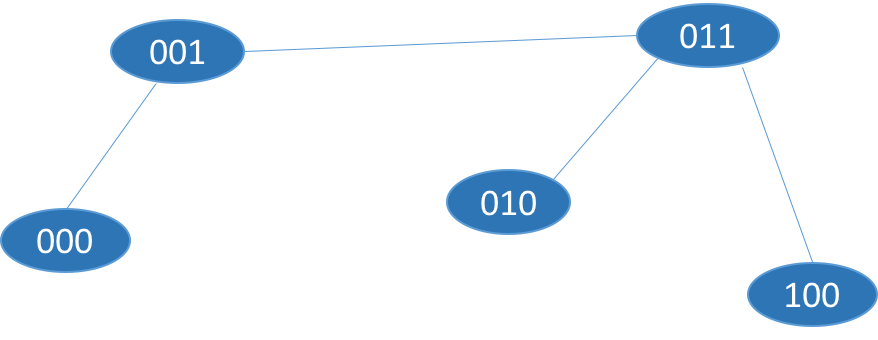
\includegraphics[width=0.5\textwidth]{Pic/1.png}
	\caption{Step 1: Encode each node in binary.}
	\label{fig:1}
\end{figure}
\subsubsection*{Step 2} For each edge $e=\{x,y\}\in E$, assign a label $l(e)=x_by_b$ to it. See Figure~\ref{fig:2} for a clearer view.
\begin{figure}[h]
	\centering
	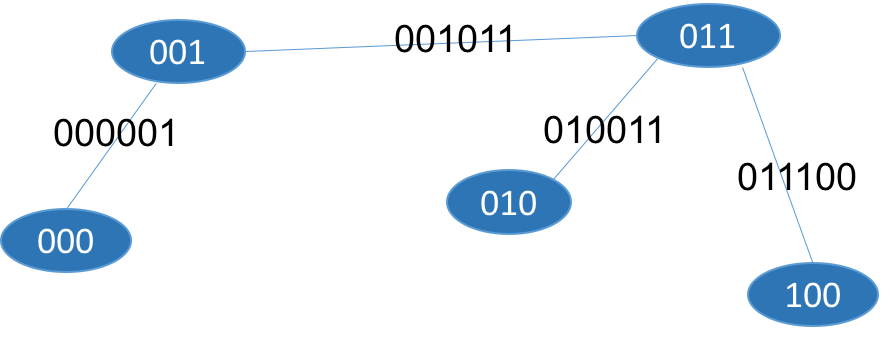
\includegraphics[width=0.5\textwidth]{Pic/2.png}
	\caption{Step 2: Assign a label to each edge.}
	\label{fig:2}
\end{figure}
\subsubsection*{Step 3} For each node $x \in V$, assign a value $v(x)=\sum_{e=\{x,y\}}l(e).$ Since the labels are represented in binary form, we can check that the summation is simply equivalent to the $XOR$ value of all these labels:
\begin{equation}
v(x)=\sum_{e=\{x,y\}}l(e)=XOR_{e=\{x,y\}l(e).}
\end{equation}
From Figure~\ref{fig:3} we can see the value of each node.
\begin{figure}[h]
	\centering
	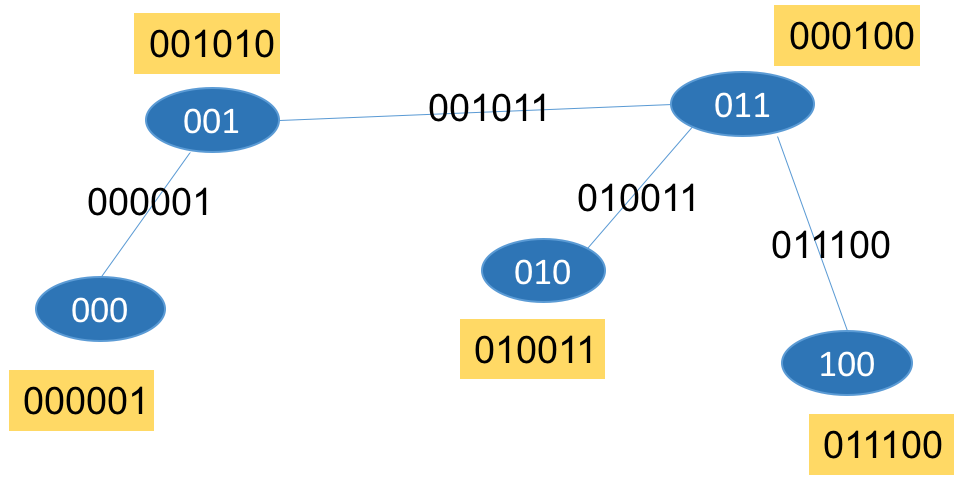
\includegraphics[width=0.5\textwidth]{Pic/3.png}
	\caption{Step 3: Assign a value to each node.}
	\label{fig:3}
\end{figure}
\subsubsection*{Step 4} For each $T \subset F$, maintain a corresponding Euler Tour Tree, with value $v(x)$ stored in Euler Tree nodes. Thus every time we call $Make\{x,y\}$ $a$ $tree$ $edge$, we link those two ET trees together using the edge $\{x,y\}$ in $O(log^3n)$ time.
\begin{figure}[h]
	\centering
	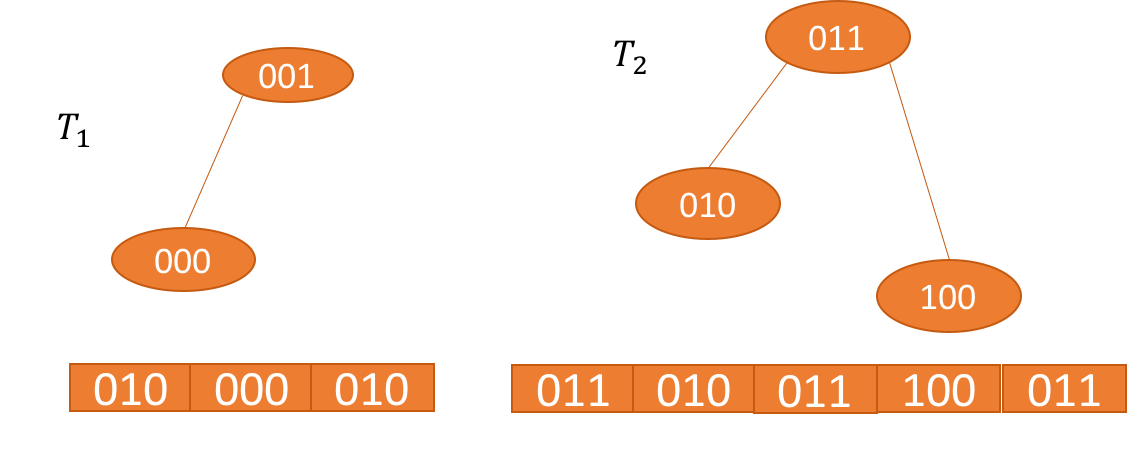
\includegraphics[width=0.5\textwidth]{Pic/4.png}
	\caption{Step 4: Construct ET trees.}
	\label{fig:4}
\end{figure}
\subsection{Fast operation implementations on cutset data structure}
\subsubsection*{One-edge case}
The data structure works mainly because of the following lemma.\\
\textit{LEMMA 2.1:The sum of the values in any tree $T$ is 0, when all the edges in $G$ incident to the tree have both endpoints in $T$; If one edge has only one endpoint in the tree, the sum of the values for the tree will reveal the label of the edge.}\\
The lemma can be verified by simple observation.
\begin{figure}[H]
	\centering
	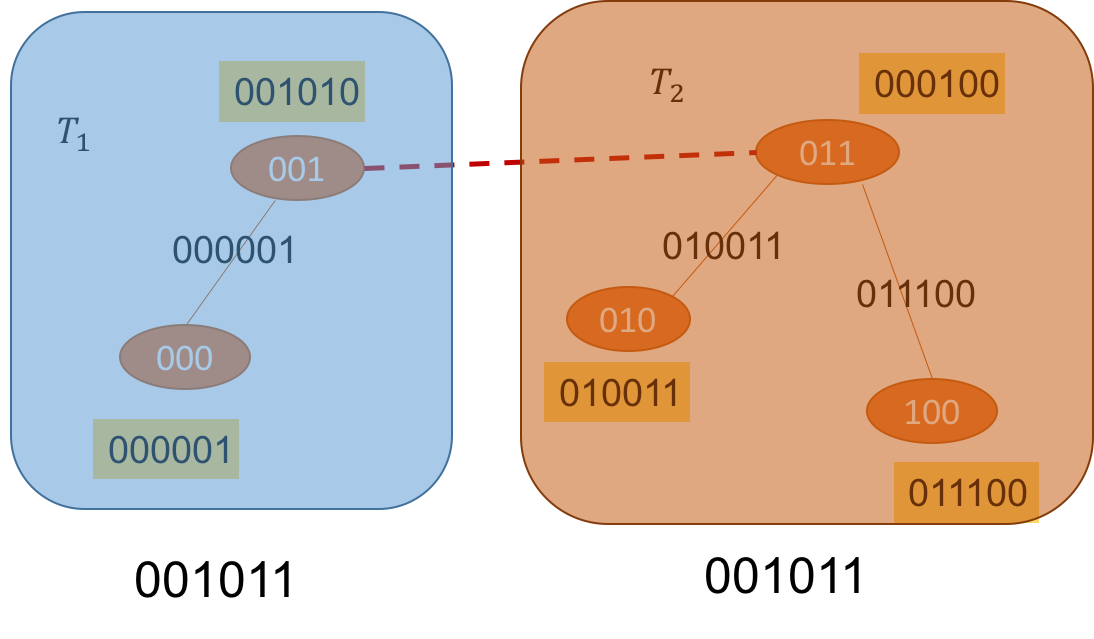
\includegraphics[width=0.5\textwidth]{Pic/5.png}
	\caption{ Illustration of lemma 2.1.}
	\label{fig:5}
\end{figure}
From Figure~\ref{fig:5}, if we sum up all the values of nodes $x \in T_1$, the result $001011$ corresponds to the label of edge $\{1,3\}$, which is the cut edge of $(T_1,T_2)=(T_1,V\backslash T_1)$. Therefore, the implementations:\\\\
$Insert\{x,y\}$: Add the edge to $G$ by adding $x_by_b$ to the value at nodes $x$ and $y$.\\\\
$Make \{x,y\}$ $a$ $tree$ $edge$: Use $\{x,y\}$ to link the ET-trees $T(x)$ and $T(y)$ in $F$.\\\\
$Delete\{x,y\}$: Subtract $x_by_b$ from the value at the node $x$ and $y$. If the edge is in $F$, remove it from $F$. Note that subtraction can be also realized by simple XOR operation.\\\\
$Search(T)$: Let $z=XOR_{x\in T}v(x)$. If $z \neq 0$, return the edge $\{z^1,z^2\}$ where $z^1$ is the first $\lceil lgn \rceil$ bits of $z$ and $z^2$ is the last $\lceil lgn \rceil$ bits of $z$.
\subsubsection*{Extension to general case} 
The problem of general cases where each cutset might contain more than one edge is that the simple $XOR$ operation cannot give the correct solution, since all these labels of cut edges would mix up with each other:
\begin{figure}[H]
	\centering
	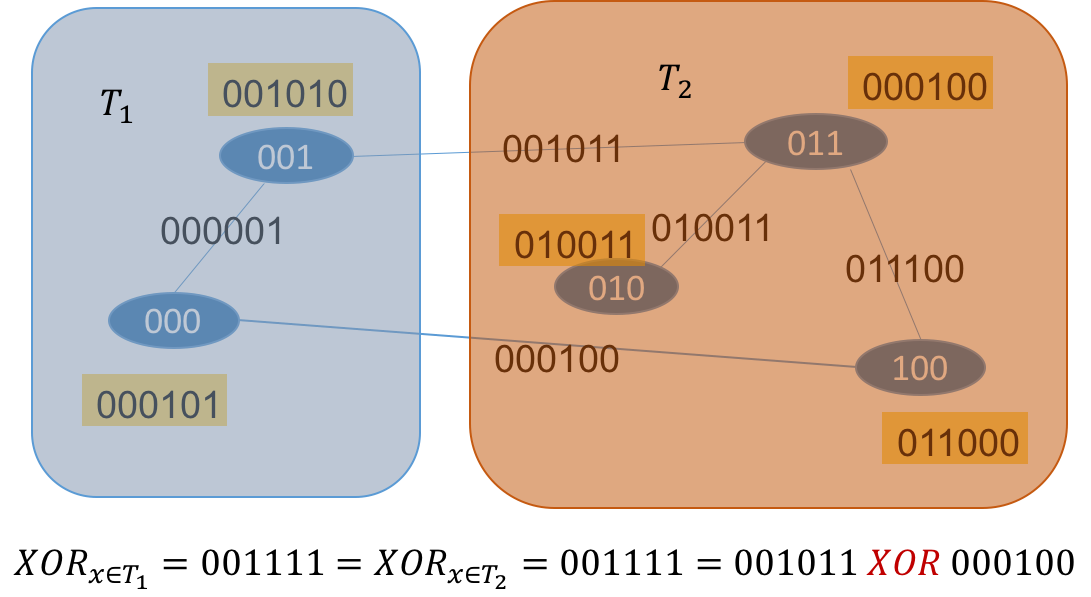
\includegraphics[width=0.5\textwidth]{Pic/6.png}
	\caption{Cut edges 'mix up' with each other.}
	\label{fig:6}
\end{figure}
The paper dealt with this problem by ensuring 
\begin{equation}
Pr(\sum_{x\in T} v(x)\textit{ gives the cut edge})=const.
\end{equation} 
To do this, the authors introduced two new concepts: \textit{level i} and \textit{version j}, where level represents an approximation of cutset size and version is used for replication. Finally there will be $\lceil 2lgn \rceil$ levels and $c'lgn$ versions in total. For simplicity, we fix the version first and consider only the level.\\
For each node $x\in V$, we maintain an array $S=\{s_0(x),s_1(x),\dots,s_{\lceil 2lgn \rceil-1}(x)\}$. Initially all entries of this array are 0, and we apply initialization of graph $G=(V,E)$ by continuously apply $Insert$ operations. While calling $Insert\{x,y\}$ operation, for each entry of array $S$, add $x_by_b$ to both $s_i(x)$ and $s_i(y)$ with a probability $\frac{1}{2^i}$, where $2^i$ is an approximate size for the cutset. The approximate size of cutset varies from 1 to approximately $\frac{n^2}{2}$, when $i$ goes from $0$ to $\lceil 2lgn \rceil-1$. This rule will lead to a good outcome that satisfies equation (2). To be specific:
\begin{proof}
As stated in lemma 2.1, if one edge $e=\{x_1,x_2\}$ has both it's endpoints inside $T$,  it won't change the value of $\sum_{x\in T} v(x)$, since it equally contributes to $x_1, x_2$ thus it would be cancelled when we apply the summation. Meanwhile, if $e$ has both it's endpoints outside $T$, it certainly will not effect the summation, either. Therefore, we only need to consider the case where $e=\{x,y\} \textit{ s.t. } x\in T, y \in (V\backslash T)$.\\\\ Suppose currently the cutset of $(T,V\backslash T)$ is $C$, where $|C|=k>1$, we check for $S[i'],i'=\lfloor lgk\rfloor$, which represents the approximate custset size $2^{\lfloor lgk\rfloor} \approx |C| $. Only when there is exactly one edge out of those all $k$ cut edges is added to both $s_{i'}(x)$ and $s_{i'}(y)$ will $\sum_{x\in T} v(x)$ give the correct result, since in this case they do not mix up. This probability is just the probability that exactly 1 out of k coinflips is heads, where each heads have probability $\frac{1}{2^{i'}}$. Note the event:$\sum_{x\in T} v(x)$\textit gives the cut edge as $E$, we have:
$$Pr(E)={k \choose 1}(\frac{1}{2^{i'}})(1-\frac{1}{2^{i'}})^{k-1} = const.$$
\end{proof}
Since equation (2) holds, we can increase the probability of correctness by repeating the process for enough times. The result of whether adding $x_by_b$ to both $s_{i1}(x)$ and $s_{i1}(y)$ will not effect that of adding $x_by_b$ to both  $s_{i2}(x)$ and $s_{i2}(y)$, i.e. these events are independent, thus by multiplication principle, if we repeat for $j=1,\dots,c'lgn$ times, the probability of all the events $E_j$ are false is at most $\Pi_{j=1}^{c'lgn}(1-E_j)$. Since $E_1=E_2=\dots=E_{c'lgn}=E$, the probability will not exceed $(1-E)^{c'lgn}$. By finding a lower bound of $E$, it is possible to choose an appropriate $c'$ such that the false negative error rate becomes quite low.
\subsection{Some discussion about cutset data structure}
\subsubsection*{Limitation}One core assumption that ensures a high accuracy rate of cutset data structure is that cutset queries and edge updates are not correlated with the random bits in the array. If it is not the case, the algorithm would fail. One simple example is that if the adversary is told the replacement edge, then he can cause the algorithm to fail by simply deleting the replacement edge after every update. After $O(log^2n)$ deletions, there will be no more replacement edges in this data structure, thus the algorithm fails.
\subsubsection*{Proof improvement} In the paper our team has been focusing on, the authors used inequality scaling to prove that $Pr(E) \ge \frac{1}{9}$ and in a further paper they tighten the bound to $Pr(E) \ge \frac{1}{8}$ by using another method(See \cite{article}). The inequality scaling goes like this:
$$Pr(E)={k \choose 1}(\frac{1}{2^{i'}})(1-\frac{1}{2^{i'}})^{k-1} > (1-\frac{1}{2^{i'}})^{2^{i'+1}}$$
By plotting them on Matlab, we find out that it is actually possible to tighten the lower bound higher:
\begin{figure}[H]
	\centering
	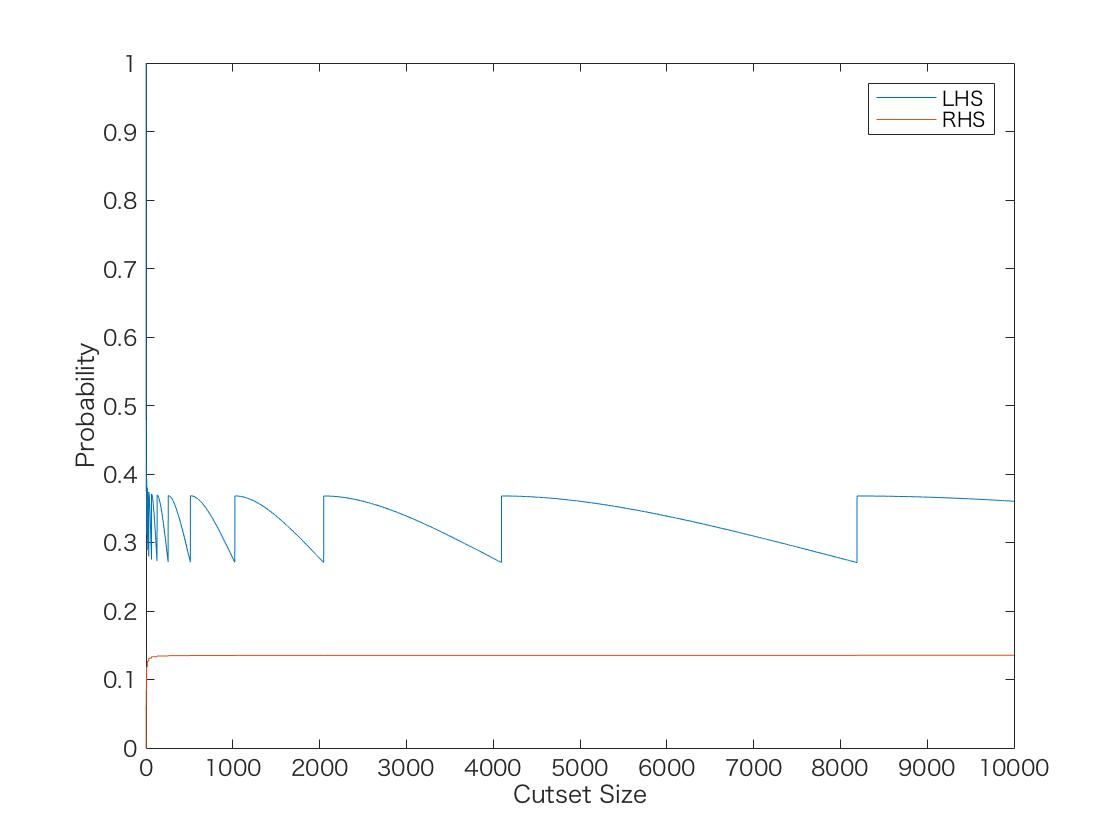
\includegraphics[width=0.5\textwidth]{Pic/fig.jpg}
	\caption{ variation of probabilities, related to cutset size.}
	\label{fig:7}
\end{figure}


\section{Fully Dynamic Connectivity}
\subsection{Why Using Boruvka tree}
Ideally, we would like to maintain a spanning forest. When a tree edge is deleted, we would query the cutset induced by one component of the broken tree and use this to find a replacement edge. This may not work because the probabilistic analysis we present will be erroneous if the possible cutset queries and the edge updates are correlated with the random bits in the array. That is, if the random bits in the array
causes certain edges to be inserted into a spanning forest, this will induce certain cutsets to be possibly considered later. It may be that the success in finding an edge in the cutset is inversely correlated with the probability that this cutset is selected.\\ A particularly
clear example is if the adversary is told the replacement edge then the adversary can cause the algorithm to fail by simply deleting the replacement edge after every update. After $O(log2 n)$ deletions, a cut would have no more replacement edges in the data structure and the
algorithm would fail.\\
We develop an algorithm which circumvents this
problem by making sure the randomness which determines
a cut is different from the randomness needed to
find an edge in the cutset.\\
So we need to use Boruvka tree algorithm to implement this.
\subsection{Boruvka tree property}
	We may view the Boruvka algorithm as constructing a sequence of tiers. On tier $l$ are the trees formed when for each tier $l−1$ tree an edge is picked linking it to another $l−1$ tree, while edges which form cycles are discarded. It's easy to see there are at most
	$\lceil lg n\rceil$ tiers.As the graph is updated, the random bits on tier $l$ are used to pick edges to join the trees from tier $l$ to form trees on tier $l + 1$.
	\begin{enumerate}
\item Let $top = \lceil lg n\rceil$, we maintain a cutset for $G$ with a forest $F_L$ for each tier. For each
tier $l$ , there is an independently generated random bit
array.
\item tier $l$ component: T, where T is tier $l$ tree formed by two(or more) $l-1$ tree and an edge(or more). And T can be represent as a tier $l$ node in Boruvka tree.
\item tier $l$ edge: Given an edge $e$, let $l$ be the minimum tier
such that $e \in F_l$
\item $unmatched$ If a node in Boruvka tree has no sibling and has not been marked as maximal, then it's unmatched.
\end{enumerate}

\subsection{Invariants}
\begin{enumerate}
	\item The tier 0 nodes of the Boruvka tree (or forest) are the vertices of G
	\item On each tier $l$, $F_l \subseteq F_{l+1}$. A tier $l + 1$ node in the Boruvka tree represents the tree obtained by linking the trees of its children with tier $l + 1$ edges
	\item Every internal node of the Boruvka tree that does not correspond to the spanning tree of a maximally connected component has at least one sibling;
	\item The structure of the forest on tier $l$ is independent of the random bits in tiers $l$ and higher.
\end{enumerate}

\section{Algorithms}
For each tier $l$ of the tree, we create
an array $S^l = s_{i,j}^l(x)$ for $x$ a vertex of G, $0 \leq
i \leq 2 lg n$ and $1 \leq j \leq c lg n$.
\subsection{Initialization}
We initialze by first creating, for each tier $l = 0, 1,2, \dots , top$, a cutset data structure where $F_l$ contains n trees consisting of the single vertices in G. we insert each edge in G using the procedure for handling edge insertions described below. And we mark $F_{top}$ as maximal to avoid unmatch.
\subsection{Handling insertions}
To insert an edge {x, y}, we first insert it into all cutset data structure on each tier. If it connects two unconnected trees in $F_{top}$, add it to $F_l$ for all $l > k$ where k is the tier of this edge.
\subsection{Handling queries}
Given a query {x, y}, if $T(x) = T(y)$ in $F_{top}$, return “yes”, else return “no”.
\subsection{Handling deletions}
\begin{algorithm}[H]
\caption{Delete\{x,y\}}
\begin{algorithmic}[1]
\State delete \{x,y\} from all CutSet.
\State delete \{x,y\} from all tree containing it.
	\For{$u \in \{x,y\}$}
		\While{u has an unmatched ancestor in the Boruvka tree}
			\State $A \gets$ the lowest unmatched ancestor of u
			\State $k \gets$ (tier of A)
			\State Reconnect(A,k)
		\EndWhile
	\EndFor


\end{algorithmic}
\end{algorithm}
\begin{algorithm}
\caption{Reconnect(A,k)}
\begin{algorithmic}[1]
\State $e = {v,w} \gets search(A,S^k)$
	\If{e = null}
		\State Mark A as maximal
	\Else
		\If{there is a path from v to w in $F_{top}$}	
			\State $e' \gets$ an edge of maximum tier on the path between v and w.
			\State Remove $e'$ from all $F_l$ that contain it
		\EndIf
		\State Add $e$ to $F_{k'}$ for all $k' > k$
	\EndIf


\end{algorithmic}

\end{algorithm}
\subsection{Details for reconnection}
We maintain a link-cut tree of $F_{top}$, the link-cut tree has the same vertexes with $F_{top}$, but the weight of edge is the edge's tier.
Then we can find the maximum tier on the path between v and w in $log(n)$ time.\\
ST-trees(link cut tree) provide a means of finding the maximum weight edge on a path between two nodes in a dynamic tree, in O(log n) time per tree edge link, cut, and the find operation.\\
Any call to Delete will result in at most $2 · top$ calls to Reconnect.
\section{Runtime Analyze}
The total cost of initialization without any edges is $O(n· top)$. The total cost of a deletion update is $O(log^5 n)$. The cost of an insertion update is $O(log^4 n)$. The cost of a query is $O(log n/ log log n)$.\\
\subsection{Deletion}
When we delete a tree edge, there may be at most $2 · top$ calls to Reconnect.Each Reconnect requires one search, and up to log $n$ links and cuts; the first costs $O(log n)$.Each link and cut of a tree storing $O(log^2 n)$ words per node costs $O(log^3 n)$ so the total cost of linking and cutting per Reconnect is $O(log^4 n)$\\
Each search requires a total cost of $O(log^3 n/ log log n)$, since it involves the testing of up to $log n$ versions each containing
$log n$ edges. Each test requires $log n/ log log n$ time to check. Since there are no more than two Reconnects per tier, the overall cost is $O(log^5 n)$
\subsection{Insertion}
An edge insertion requires an insertion into $log n$ cutset
data structures. Each costs $O(log^3 n)$ for a total of
$O(log^4 n)$. If the edge becomes a tree edge, it is inserted
into trees in $log n$ tiers, for a cost of $O(log^3 n)$ per tier
or $O(log^4 n)$ overall.
\subsection{Query}
The query time is $O(log n/ log log n)$ using degree $log n$ ET-trees


\section{Application}
	\subsection{Emergency Planning}
		\par Emergency Planning is one the applications of such algorithm. Given a graph $G$, the problem is to be able to prepross G so that structural information can be returned regardless online insertions and deletions.
		\par There have been work on this problem\cite{abboud2014popular} who relies on $\gamma$-approximation and gives an $O(\gamma d \log^2n\log\log n)$ worse case update time and $O(\log \log n)$ query time.
		\par We can use this data structure to construct a spanning forest, store this forest in a balanced complete ET tree and insert using dynamic connectivity edge insertion algorithm. 
		We can give us a cost of $O(d\log^3 n \log d)$ for update and $O(\log n)$ for query.
		However, to reduce time complexity to $O(\log \log n)$, we follow ideas proposed in \cite{abboud2014popular}. 
	\subsubsection{Even Faster}
		\par We can cut down the amount of work in this algorithm by limiting the number of versions to $O(1)$, thus finding a replacement in a cutset problem requires an expected constant number of versions checked, instead of $O(\log n)$. Considering the fact that there are $O(\log n)$ levels, we can not find it even faster.
\section{Discussion}
	\subsection{Errors in the paper}
	\subsection{Future}
		\par Unlike other work trying to tackle dynamic graph, this work introduced a new method for adaptive graph sketching with a concern for fast update and query time. 
		However, it's interesting to ask the fastest update and query time for other dynamic graph problems?
		\par Classic dynamic graph problems are dynamic minimum spanning tree in $o(\sqrt{n})$ worst case time and Las Vegas or deterministic graph connectivity with $o(\sqrt{n}$ worst case cost.

\bibliographystyle{IEEEtran}
%% De-comment this line if you have any reference.
%% And don't forget to change .bib file.
\bibliography{report}
\end{document}
